\documentclass{article}
\usepackage[utf8]{inputenc}
\usepackage[T1]{fontenc}
\usepackage[polish]{babel}
\usepackage[a4paper, margin=1in]{geometry}
\usepackage{multicol}
\usepackage{amsmath}
\usepackage{gensymb}
\usepackage{graphicx}
\usepackage{multirow}
\usepackage{array}
\usepackage{caption}
\usepackage{float}
\usepackage{hyperref}
\usepackage{karnaugh-map}
\usepackage{tikz}
\usepackage[linesnumbered,ruled,vlined]{algorithm2e}
\usepackage{pgfplotstable}
\usepackage{booktabs}
\pgfplotsset{compat=1.18}

\begin{document}

\begin{multicols}{3}
    \begin{figure}[H]
        
\includegraphics[scale=0.4]{jpg/DOJEBANE_LOGO_PWR.png}
        \label{fig:enter-label}
    \end{figure}
    
    \begin{figure}[H]
    \end{figure}
    
    \begin{figure}[H]
        
\includegraphics[scale=0.4]{jpg/w4n.png}
        \centering
        \textbf{W4N}
        \label{fig:WYDZIAŁ INFORMATYKI I TELEKOMUNIKACJI}
    \end{figure}
\end{multicols}

\vspace{75pt}

\begin{center}
    \textbf{\large Badanie efektywności algorytmów grafowych w zależności od rozmiaru instancji oraz sposobu
reprezentacji grafu w pamięci komputeraą} 
    \vspace{2pt}
    \hrule
    \vspace{4pt}
    \textbf{\large Algorytmy i złożoność obliczeniowa - Projekt} 
\end{center}

\vspace{75pt}

\begin{center}
    \textbf{Autor: } \\
    Filip Kwiek 280947
\end{center}

\begin{center}
    \textbf{Termin zajęć: } \\
    Wtorek np. 11:15
\end{center}

\begin{center}
    \textbf{Prowadzący: } \\
    Dr. inż. Jarosław Mierzwa
\end{center}

\newpage
\tableofcontents
\newpage

\section{Wstęp}
Celem projektu było zbadanie efektywności wybranych grafowych:

\begin{itemize}
    \item Algorytmów minimalnego drzewa rozpinającego (MST)
    \item Algorytmów najkrótszej ścieżki
    \item Algorytmów maksymalnego przepływu
\end{itemize}

W projekcie dla każdego problemu badam czas wykonania algorytmu w zależności od rozmiaru instancji oraz sposobu reprezentacji grafu w pamięci komputera.
Wszystkie algorytmy zostały zaimplementowane w języku C++ i przetestowane na losowo wygenerowanych grafach o różnych gęstościach oraz reprezentacjach.

Wybrane algorytmy grafowe:
\begin{itemize}
    \item Algorytm Kruskala
    \item Algorytm Prima
    \item Algorytm Dijkstry
    \item Algorytm Bellmana-Forda
    \item Algorytm Forda-Fulkersona
    \item Algorytm Edmondsa-Karpa
\end{itemize}

\section{Technologie użyte w projekcie}
Projet został wykonany w języku c++ w wersji 20. Do kompilacji użyto kompilatora g++ w wersji 14.2.1, 
a do zbudowania oraz zarządzania strukturą wykorzystano system CMake w wersji 3.30
Do zapisu oraz odczytu plików wykorzysano bibliotekę $fstream$, natomiast do pomiaru czasu bibliotekę $chrono$.

\section{Plan eksperymentu}

W ramach przygotowań, cały plan oparty został na założeniu, iż grafy są generowane losowo niezależnie dla każdej reprezetacji, jednocześnie mając stały rozmiar 1000 węzłów.

Eksperyment będzie polegał na zmierzeniu czasu wykonywania algorytmu na 5 reprezentatywnych gęstościach grafów:
\begin{itemize}
    \item 20\%
    \item 60\%
    \item 99\%
\end{itemize}

7 reprezentatywnych rozmiarach grafów:

\begin{itemize}
    \item 100 węzłów
    \item 250 węzłów
    \item 300 węzłów
    \item 400 węzłów
    \item 500 węzłów
    \item 600 węzłów
    \item 800 węzłów
\end{itemize}

Oraz na 2 reprezentacjach grafów:
\begin{itemize}
    \item Lista sąsiedztwa
    \item Macierz sąsiedztwa
\end{itemize}

Dla każdej gęstości oraz reprezentacji grafu zostało wykonane 10 pomiarów czasu, a dane obejmują ich średnią z każdego pomiaru.

Podczas pomiarów, dane były zapisywane do plików csv. Ze względu na ich ilość, nie zostały one wrzucone razem z kodem, ale istnieje możliwość ich samodzielnej generacji w programie.
Przy opisie grafów, nie uwzględniam ich złożoności pamięciowej ponieważ zależy ona od ich reprezentacji, a nie od gęstości grafu. 

Złożoności pamięciowe dla obu reprezentacji są następujące:
\begin{itemize}
    \item Macierz sąsiedztwa: $O(V^2)$, gdzie $V$ to liczba wierzchołków w grafie.
    \item Lista sąsiedztwa: $O(V + E)$, gdzie $E$ to liczba krawędzi w grafie.
\end{itemize}

\section{Użyty sprzęt}

\begin{itemize}
    \item Procesor: Amd Ryzen 5 3550H 2.1GHz
    \item Pamięć RAM: 32GB DDR4
    \item System operacyjny: EndeavourOS (Arch Linux) - kernel 6.14.7-zen2-1-zen
\end{itemize}

Podczas pomiarów sprzęt był używany na zasilaniu sieciowym, a proces nie był przypisany do jednego rdzenia, przez aplikację $irqbalance$, która rozbija na siłę procesy
obciążające jeden rdzeń na wszystkie rdzenie procesora. Ponadto taktowanie procesora nie było ustawione na stałe.

\section{Problem MST}

Problem minimalnego drzewa rozpinającego (MST) polega na znalezieniu podzbioru krawędzi grafu, który tworzy drzewo rozpinające i ma najmniejszą możliwą sumę wag krawędzi.
W kontekście grafów, drzewo rozpinające to podgraf, który zawiera wszystkie wierzchołki grafu i jest drzewem (czyli nie ma cykli). Minimalne drzewo rozpinające to takie drzewo, które ma najmniejszą możliwą sumę wag krawędzi spośród wszystkich możliwych drzew rozpinających.
Istnieją trzy popularne algorytmy do rozwiązania tego problemu:
\begin{itemize}
    \item Algorytm Kruskala
    \item Algorytm Prima
    \item Algorytm Boruvki
\end{itemize}

W moim eksperymencie, zastosowałem dwa pierwsze algorytmy, ponieważ są one najpopularniejsze i najczęściej stosowane w praktyce.

\subsection{Algorytmn Kruskala}

Algorytm Kruskala jest jednym z najpopularniejszych algorytmów do znajdowania minimalnego drzewa rozpinającego w grafie.
Działa on na zasadzie sortowania krawędzi grafu według ich wag i dodawania ich do drzewa rozpinającego, o ile nie tworzą cyklu. 
Algorytm ten jest szczególnie efektywny w przypadku grafów rzadkich.

\begin{itemize}
    \item Złożoność czasowa: $O(E \log E)$, gdzie $E$ to liczba krawędzi w grafie.
\end{itemize}

Moja imlementacja zakłada użycie struktury setów rozłącznych do sprawdzania cykli, co pozwala na efektywne zarządzanie zbiorami wierzchołków.

\subsubsection{Lista kroków}
\begin{enumerate}
    \item Posortuj krawędzie grafu według ich wag.
    \item Inicjalizuj zbiór rozłącznych zbiorów dla każdego wierzchołka.
    \item Iteruj przez posortowane krawędzie:
    \begin{itemize}
        \item Jeśli krawędź łączy dwa różne zbiory, dodaj ją do drzewa rozpinającego i połącz te zbiory.
    \end{itemize}
    \item Zwróć drzewo rozpinające.
    \item Zwróć sumę wag krawędzi w drzewie rozpinającym.
\end{enumerate}

\subsection{Algorytm Prima}

Algorytm Prima jest kolejnym popularnym algorytmem do znajdowania minimalnego drzewa rozpinającego w grafie.
Działa on na zasadzie iteracyjnego dodawania krawędzi do drzewa rozpinającego, zaczynając od dowolnego wierzchołka i wybierając zawsze krawędź o najmniejszej wadze, która łączy drzewo z wierzchołkiem spoza drzewa.
\begin{itemize}
    \item Złożoność czasowa: $O(E \log V)$, gdzie $E$ to liczba krawędzi, a $V$ to liczba wierzchołków w grafie.
\end{itemize}

Moja implementacja zakłada użycie kopców minimalbych, które pozwalają na efektywne zarządzanie krawędziami i ich wagami. Ulepsza to wydajność algorytmu,
ponieważ znajdywanie krawędzi o najmniejszej wadze w najgorszym wypadku będzie wynosić $O(\log V)$, a nie $O(V)$, jak w przypadku prostego algorytmu.

\subsubsection{Lista kroków}
\begin{enumerate}
    \item Inicjalizuj drzewo rozpinające jako puste.
    \item Wybierz dowolny wierzchołek jako wierzchołek startowy i dodaj go do drzewa rozpinającego.
    \item Utwórz kopiec minimalny, który będzie przechowywał krawędzie łączące drzewo z wierzchołkami spoza drzewa.
    \item Iteruj, dopóki kopiec nie jest pusty:
    \begin{itemize}
        \item Wyciągnij krawędź o najmniejszej wadze z kopca.
        \item Jeśli krawędź łączy drzewo z wierzchołkiem spoza drzewa, dodaj ją do drzewa rozpinającego i dodaj sąsiadujące krawędzie do kopca.
    \end{itemize}
    \item Zwróć drzewo rozpinające.
    \item Zwróć sumę wag krawędzi w drzewie rozpinającym.
\end{enumerate}

\section{Problem najkrótszej ścieżki}

Problem najkrótszej ścieżki polega na znalezieniu najkrótszej ścieżki pomiędzy dwoma wierzchołkami w grafie. Istnieje wiele algorytmów do rozwiązania tego problemu, ale dwa z nich są szczególnie popularne:
\begin{itemize}
    \item Algorytm Dijkstry
    \item Algorytm Bellmana-Forda
\end{itemize}

\subsection{Algorytm Dijkstry}

Algorytm Dijkstry jest jednym z najpopularniejszych algorytmów do znajdowania najkrótszej ścieżki w grafie z dodatnimi wagami krawędzi.
Działa on na zasadzie iteracyjnego znajdowania najkrótszej ścieżki do każdego wierzchołka, zaczynając od wierzchołka źródłowego i aktualizując odległości do sąsiadujących wierzchołków.
\begin{itemize}
    \item Złożoność czasowa: $O(E \log V)$, gdzie $E$ to liczba krawędzi, a $V$ to liczba wierzchołków w grafie.
\end{itemize}

Algorytm Dijkstry działa tylko dla grafów z dodatnimi wagami krawędzi. 
W przypadku grafów z ujemnymi wagami krawędzi, należy użyć algorytmu Bellmana-Forda.

\subsubsection{Lista kroków}
\begin{enumerate}
    \item Inicjalizuj odległości do wszystkich wierzchołków jako nieskończoność, a odległość do wierzchołka źródłowego jako 0.
    \item Utwórz kopiec minimalny, który będzie przechowywał wierzchołki i ich odległości.
    \item Iteruj, dopóki kopiec nie jest pusty:
    \begin{itemize}
        \item Wyciągnij wierzchołek o najmniejszej odległości z kopca.
        \item Dla każdego sąsiada tego wierzchołka, jeśli nowa odległość jest mniejsza niż obecna, zaktualizuj odległość i dodaj sąsiada do kopca.
    \end{itemize}
    \item Zwróć tablicę odległości do wszystkich wierzchołków.
    \item Zwróć najkrótszą ścieżkę do wierzchołka docelowego.
\end{enumerate}

\subsection{Algorytm Bellmana-Forda}

Algorytm Bellmana-Forda jest algorytmem do znajdowania najkrótszej ścieżki w grafie, który może zawierać krawędzie o ujemnych wagach.
Działa on na zasadzie iteracyjnego relaksowania krawędzi grafu, co pozwala na znalezienie najkrótszej ścieżki do każdego wierzchołka.
\begin{itemize}
    \item Złożoność czasowa: $O(V \cdot E)$, gdzie $V$ to liczba wierzchołków, a $E$ to liczba krawędzi w grafie.
\end{itemize}

Algorytm Bellmana-Forda jest bardziej uniwersalny niż algorytm Dijkstry, ponieważ może obsługiwać grafy z ujemnymi wagami krawędzi, ale jest mniej wydajny w przypadku grafów z dodatnimi wagami krawędzi.
\subsubsection{Lista kroków}
\begin{enumerate}
    \item Inicjalizuj odległości do wszystkich wierzchołków jako nieskończoność, a odległość do wierzchołka źródłowego jako 0.
    \item Iteruj $V-1$ razy (gdzie $V$ to liczba wierzchołków):
    \begin{itemize}
        \item Dla każdej krawędzi $(u, v)$ z wagą $w$, jeśli odległość do $u$ + $w$ jest mniejsza niż odległość do $v$, zaktualizuj odległość do $v$.
    \end{itemize}
    \item Sprawdź, czy istnieją cykle o ujemnej wadze:
    \begin{itemize}
        \item Jeśli po $V-1$ iteracjach można jeszcze zaktualizować jakąkolwiek krawędź, to graf zawiera cykl o ujemnej wadze.
    \end{itemize}
    \item Zwróć tablicę odległości do wszystkich wierzchołków.
    \item Zwróć najkrótszą ścieżkę do wierzchołka docelowego.
\end{enumerate}

\section{Problem maksymalnego przepływu}

Problem maksymalnego przepływu polega na znalezieniu maksymalnego przepływu w sieci przepływowej, która jest grafem skierowanym z dodatnimi wagami krawędzi.
Istnieją dwa popularne algorytmy do rozwiązania tego problemu:

\begin{itemize}
    \item Algorytm Forda-Fulkersona
    \item Algorytm Edmondsa-Karpa
\end{itemize}

\subsection{Algorytm Forda-Fulkersona (przeszukiwanie grafu w głąb)}

Algorytm Forda-Fulkersona jest jednym z najpopularniejszych algorytmów do znajdowania maksymalnego przepływu w sieci przepływowej.
Działa on na zasadzie iteracyjnego znajdowania ścieżek powiększających przepływ w sieci i aktualizowania przepływu, aż nie będzie już możliwe znalezienie kolejnej ścieżki powiększającej.
\begin{itemize}
    \item Złożoność czasowa: $O(E \cdot f)$, gdzie $E$ to liczba krawędzi w grafie, a $f$ to maksymalny przepływ.
\end{itemize}

Moja implementacja zakłada użycie algorytmu przeszukiwania w głąb (DFS) do znajdowania ścieżek powiększających przepływ, co pozwala na efektywne zarządzanie przepływem w sieci.
\subsubsection{Lista kroków}
\begin{enumerate}
    \item Inicjalizuj przepływ do wszystkich krawędzi jako 0.
    \item Iteruj, dopóki istnieje ścieżka powiększająca przepływ:
    \begin{itemize}
        \item Znajdź ścieżkę powiększającą przepływ w sieci za pomocą algorytmu DFS.
        \item Oblicz minimalną pojemność na tej ścieżce.
        \item Zaktualizuj przepływ wzdłuż tej ścieżki.
    \end{itemize}
    \item Zwróć maksymalny przepływ.
\end{enumerate}

\subsection{Algorytm Edmondsa-Karpa (przeszukiwanie grafu wszerz)}
Algorytm Edmondsa-Karpa jest ulepszoną wersją algorytmu Forda-Fulkersona, która wykorzystuje algorytm przeszukiwania wszerz (BFS) do znajdowania ścieżek powiększających przepływ.
Działa on na zasadzie iteracyjnego znajdowania ścieżek powiększających przepływ w sieci i aktualizowania przepływu, aż nie będzie już możliwe znalezienie kolejnej ścieżki powiększającej.
\begin{itemize}
    \item Złożoność czasowa: $O(V \cdot E^2)$, gdzie $V$ to liczba wierzchołków, a $E$ to liczba krawędzi w grafie.
\end{itemize}
Moja implementacja zakłada użycie algorytmu przeszukiwania wszerz (BFS) do znajdowania ścieżek powiększających przepływ, co pozwala na efektywne zarządzanie przepływem w sieci.
\subsubsection{Lista kroków}
\begin{enumerate}
    \item Inicjalizuj przepływ do wszystkich krawędzi jako 0.
    \item Iteruj, dopóki istnieje ścieżka powiększająca przepływ:
    \begin{itemize}
        \item Znajdź ścieżkę powiększającą przepływ w sieci za pomocą algorytmu BFS.
        \item Oblicz minimalną pojemność na tej ścieżce.
        \item Zaktualizuj przepływ wzdłuż tej ścieżki.
    \end{itemize}
    \item Zwróć maksymalny przepływ.
\end{enumerate}

\section{Przebieg eksperymentu}

Dla każdego algorytmu zastosowano dwie opisane wcześniej reprezentacje oraz gęstości grafów. 
Każdy algorytm był wykonywany na osobno losowym generowanym grafie, niezależnie od reprezentacji. 
Każdy z nich został uruchomiony 20 razy (10 dla listy sąsiedztwa i 10 dla macierzy sąsiedztwa), a czas wykonania został uśredniony. Wyniki
przedstawiono na wykresach, gdzie oś X to rozmiar tablicy, a oś Y to czas wykonania algorytmu w milisekundach.

\subsection{Problem MST}

\subsubsection{Tabele}
\pgfplotstableread[col sep=comma]{../Results/Type1_MST_type1_AdjacencyList.csv}\datatable

\begin{table}[H]
\centering
\pgfplotstabletypeset[
    columns/column1/.style={column name=Density},
    columns/column2/.style={column name=Kruskal (ms)},
    columns/column3/.style={column name=Prim (ms)},
    every head row/.style={before row=\toprule,after row=\midrule},
    every last row/.style={after row=\bottomrule}
]{\datatable}
\caption{Tabela średnich wyników w milisekundach dla algorytmu Kruskala i Prima dla Listy sąsiedztwa}
\end{table}

    

\pgfplotstableread[col sep=comma]{../Results/Type1_MST_type1_AdjacencyMatrix.csv}\datatable

\begin{table}[H]
\centering
\pgfplotstabletypeset[
    columns/column1/.style={column name=Density},
    columns/column2/.style={column name=Kruskal (ms)},
    columns/column3/.style={column name=Prim (ms)},
    every head row/.style={before row=\toprule,after row=\midrule},
    every last row/.style={after row=\bottomrule}
]{\datatable}
\caption{Tabela średnich wyników w milisekundach dla algorytmu Kruskala i Prima dla Macierzy sąsiedztwa}
\end{table}


\subsubsection{Wykresy Typu 1 dla Kruskala i Prima}

\begin{figure}[H]
    \centering
    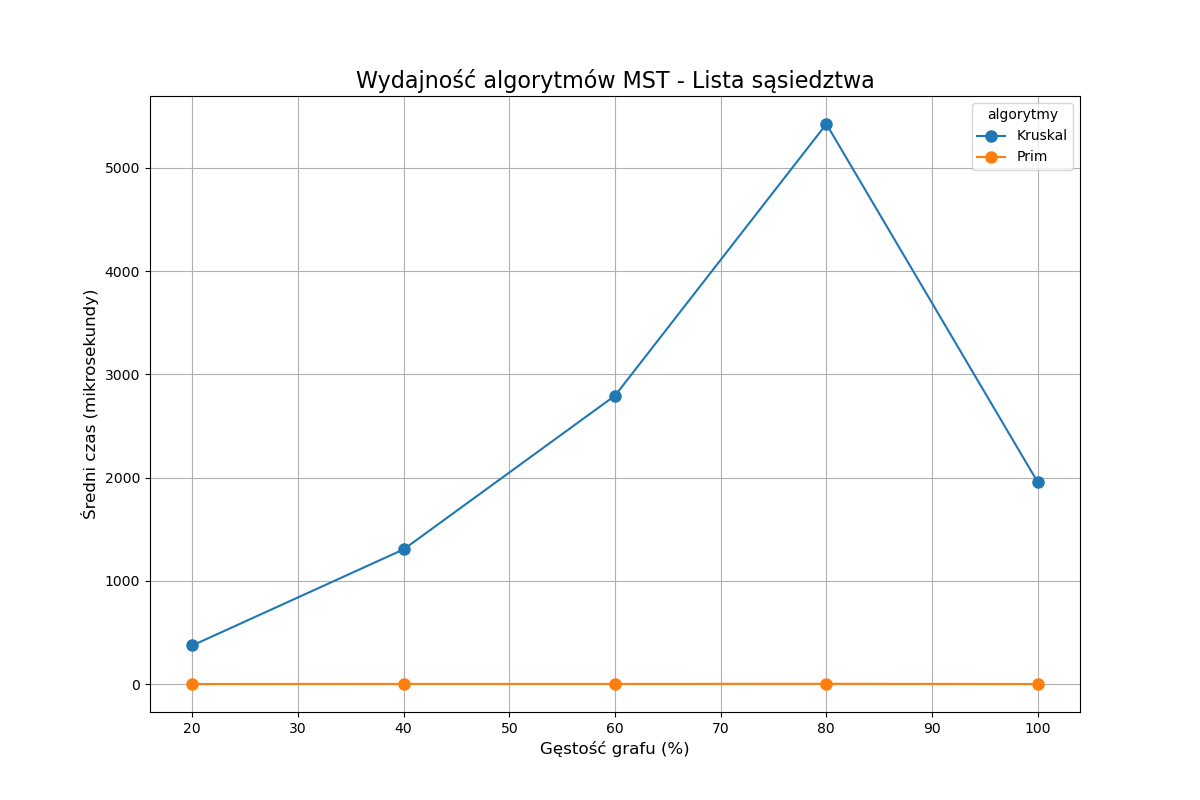
\includegraphics[scale=0.5]{../Python/charts_type1/Typ1_MST_Lista_sąsiedztwa_wykres.png}
    \caption{Czasy wykonania algorytmów Kruskala i Prima dla Listy sąsiedztwa}
\end{figure}
\begin{figure}[H]
    \centering
    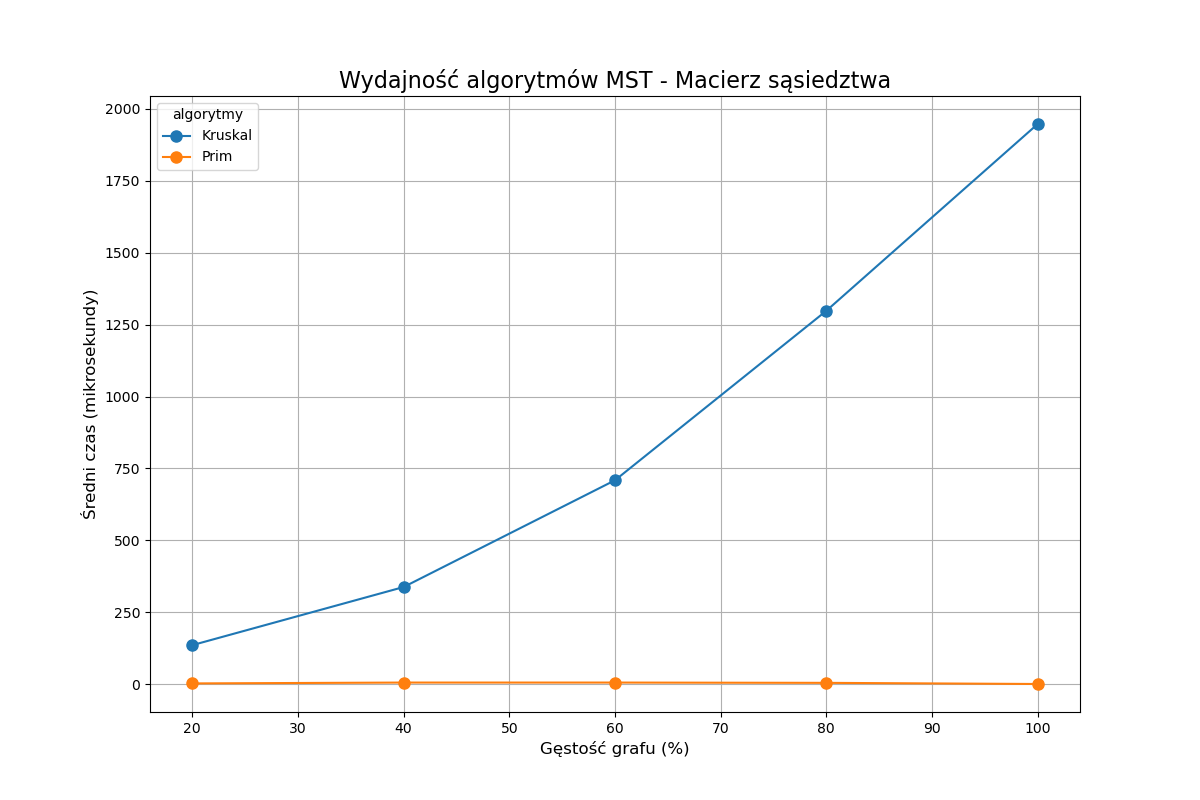
\includegraphics[scale=0.5]{../Python/charts_type1/Typ1_MST_Macierz_sąsiedztwa_wykres.png}
    \caption{Czasy wykonania algorytmów Kruskala i Prima dla Macierzy sąsiedztwa}
\end{figure}

\subsubsection{Wykresy Typu 2 dla Kruskala i Prima}

\begin{figure}[H]
    \centering
    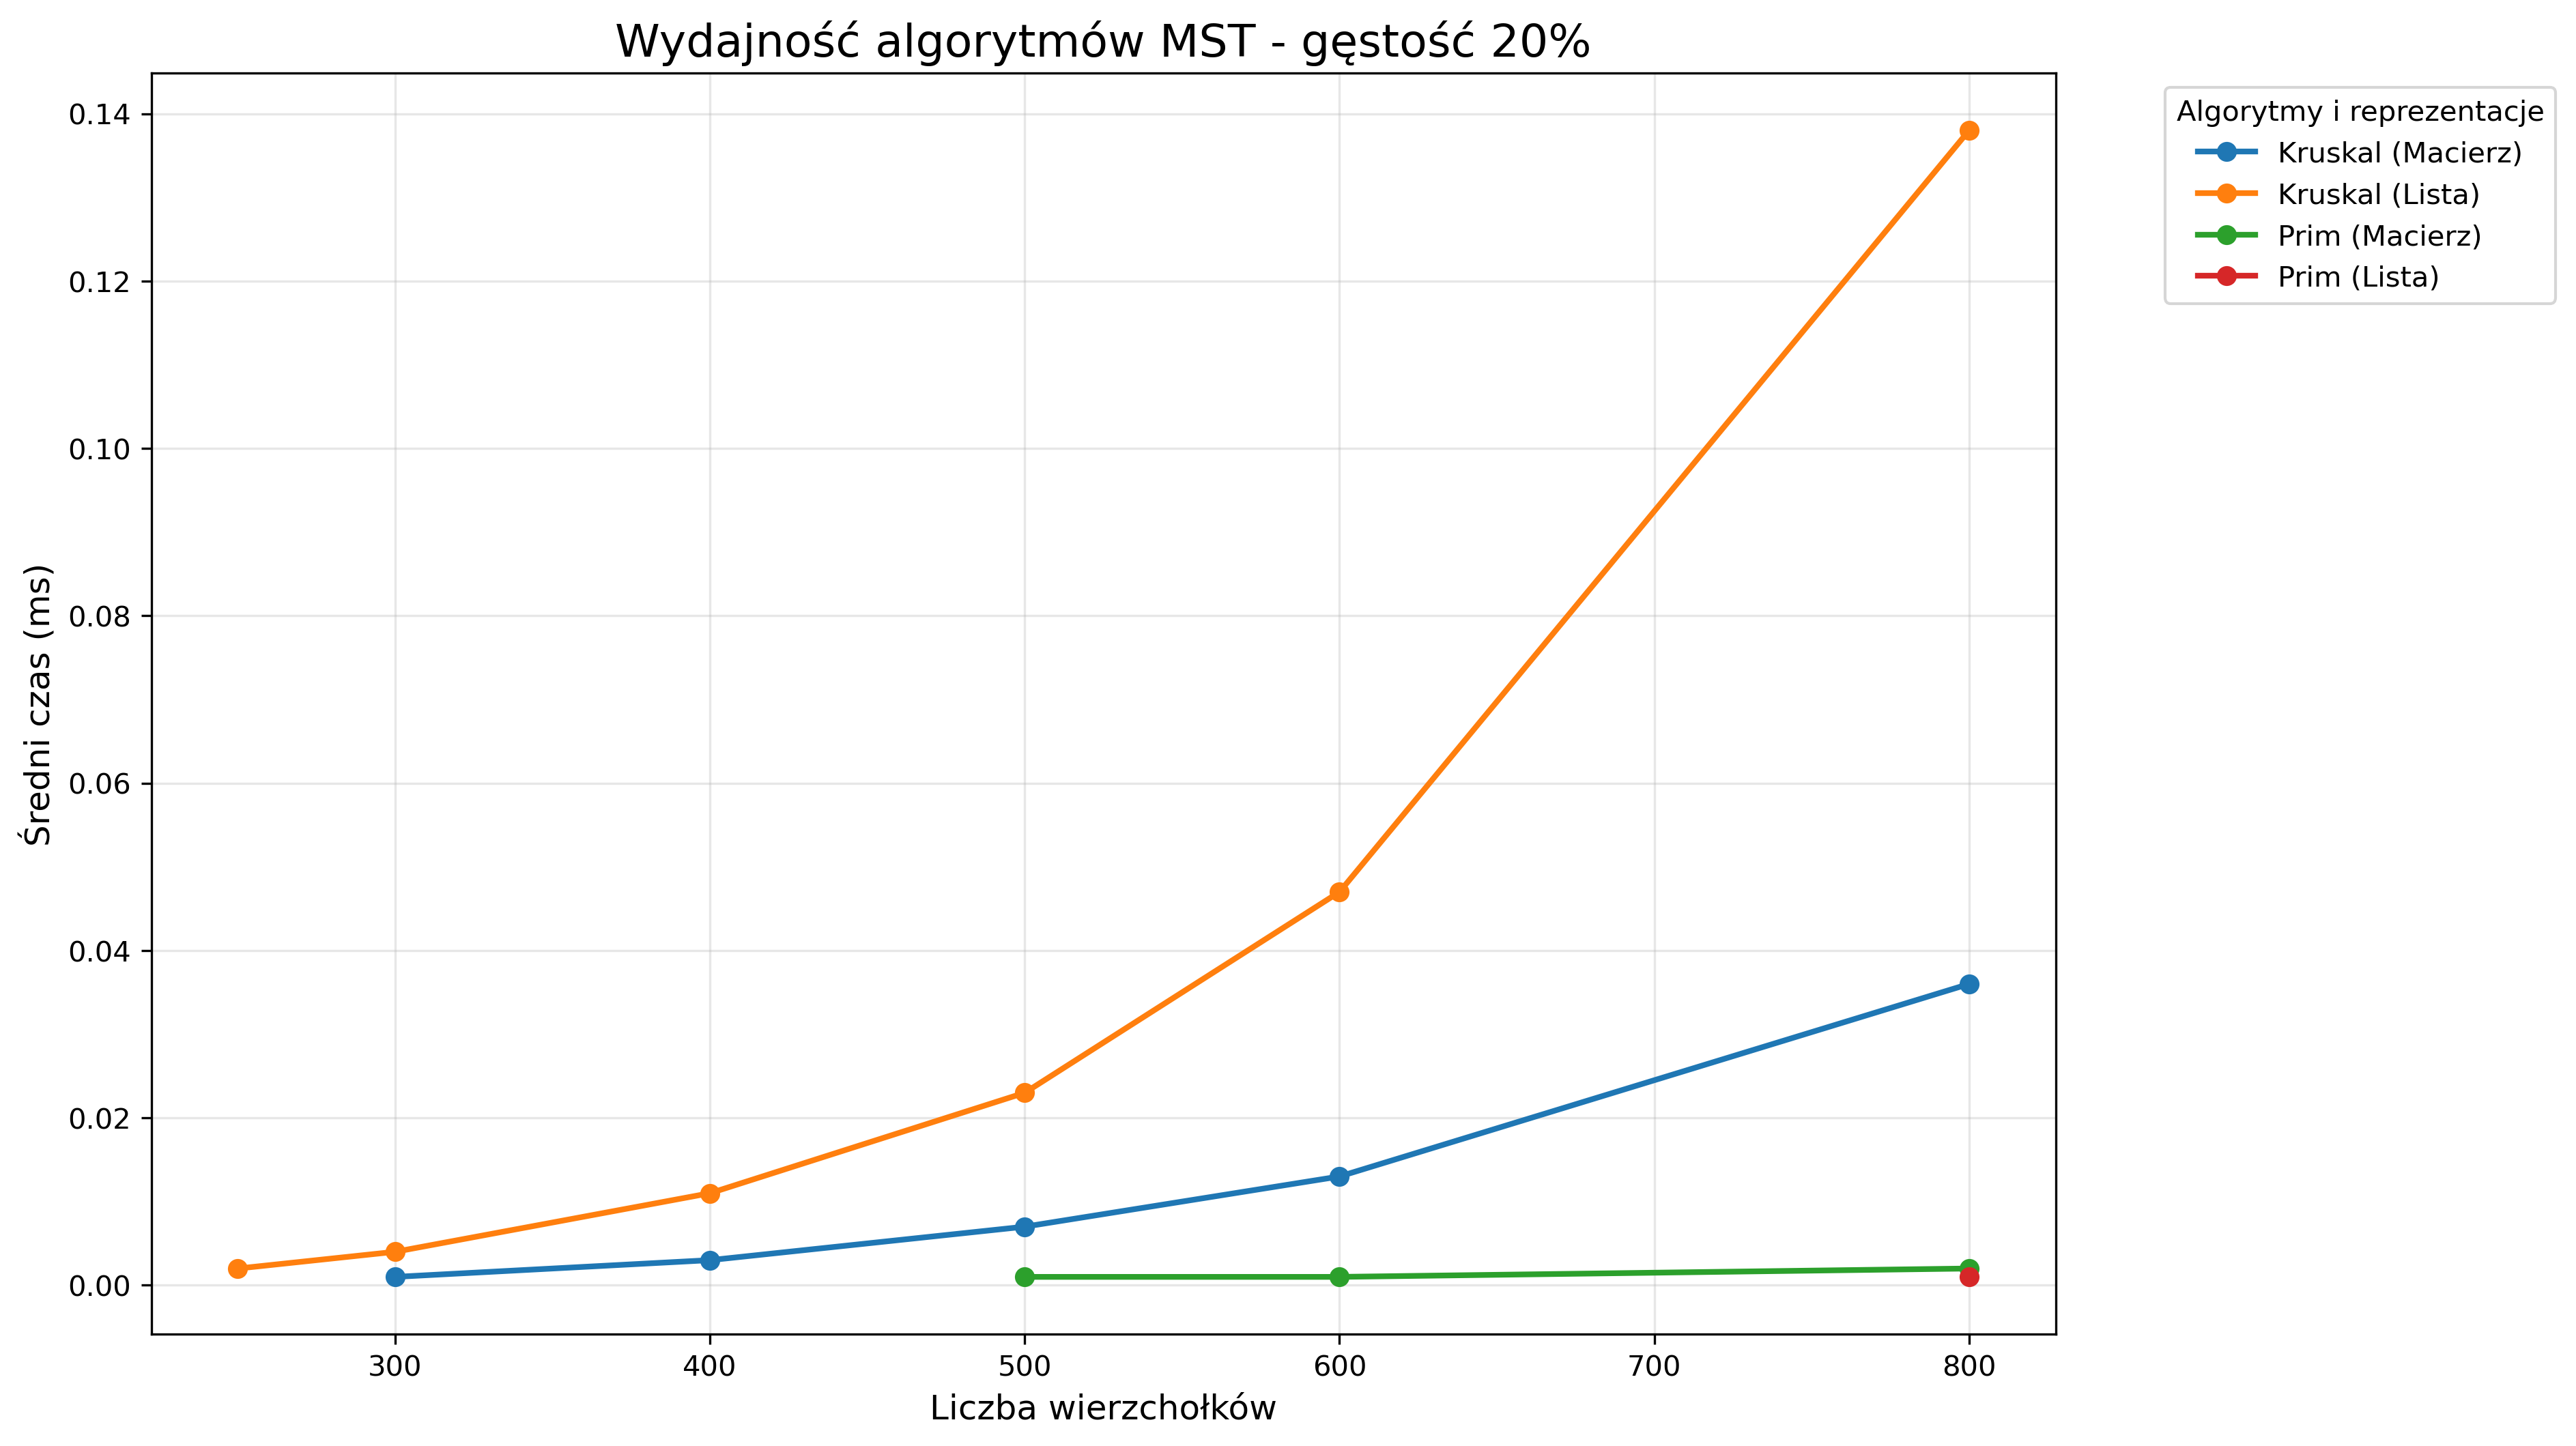
\includegraphics[scale=0.5]{../Python/charts_type2/Typ2_MST_gestosc20_wykres.png}
    \caption{Czasy wykonania algorytmów Kruskala i Prima dla gęstości 20\%}
\end{figure}
\begin{figure}[H]
    \centering
    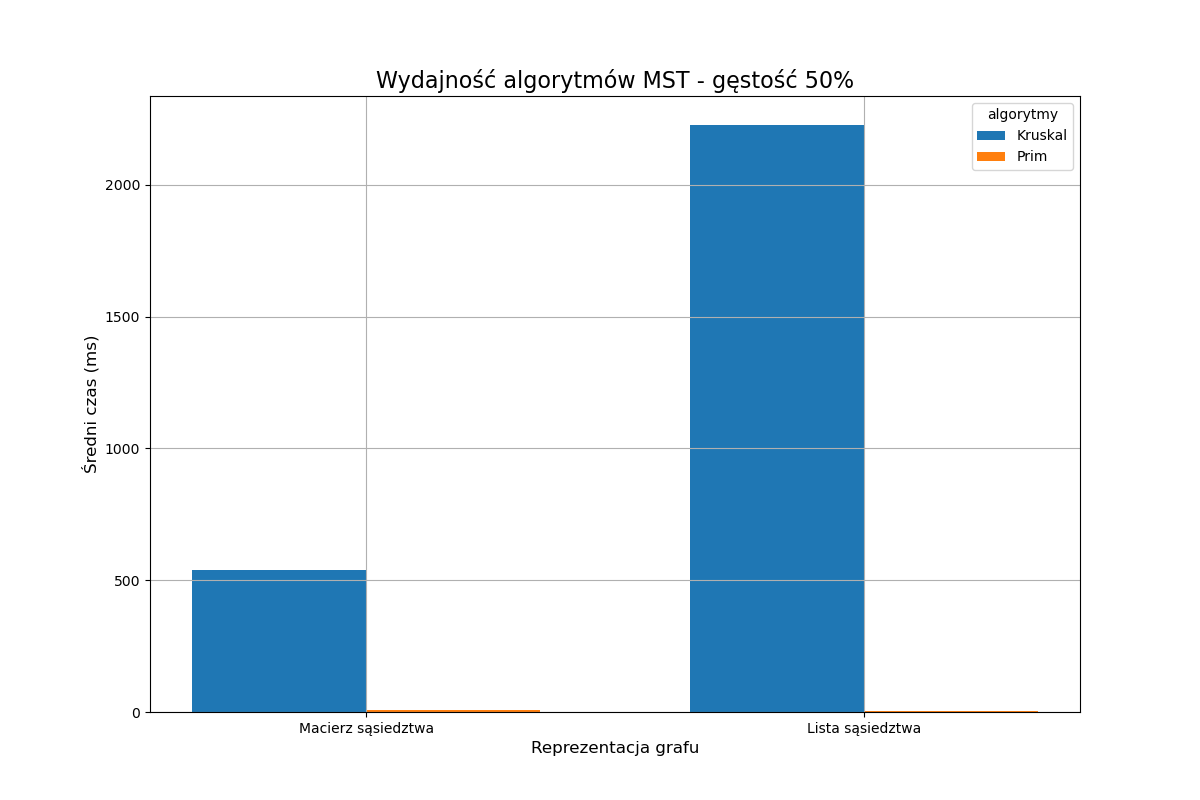
\includegraphics[scale=0.5]{../Python/charts_type2/Typ2_MST_gestosc50_wykres.png}
    \caption{Czasy wykonania algorytmów Kruskala i Prima dla gęstości 50\%}
\end{figure}

\begin{figure}[H]
    \centering
    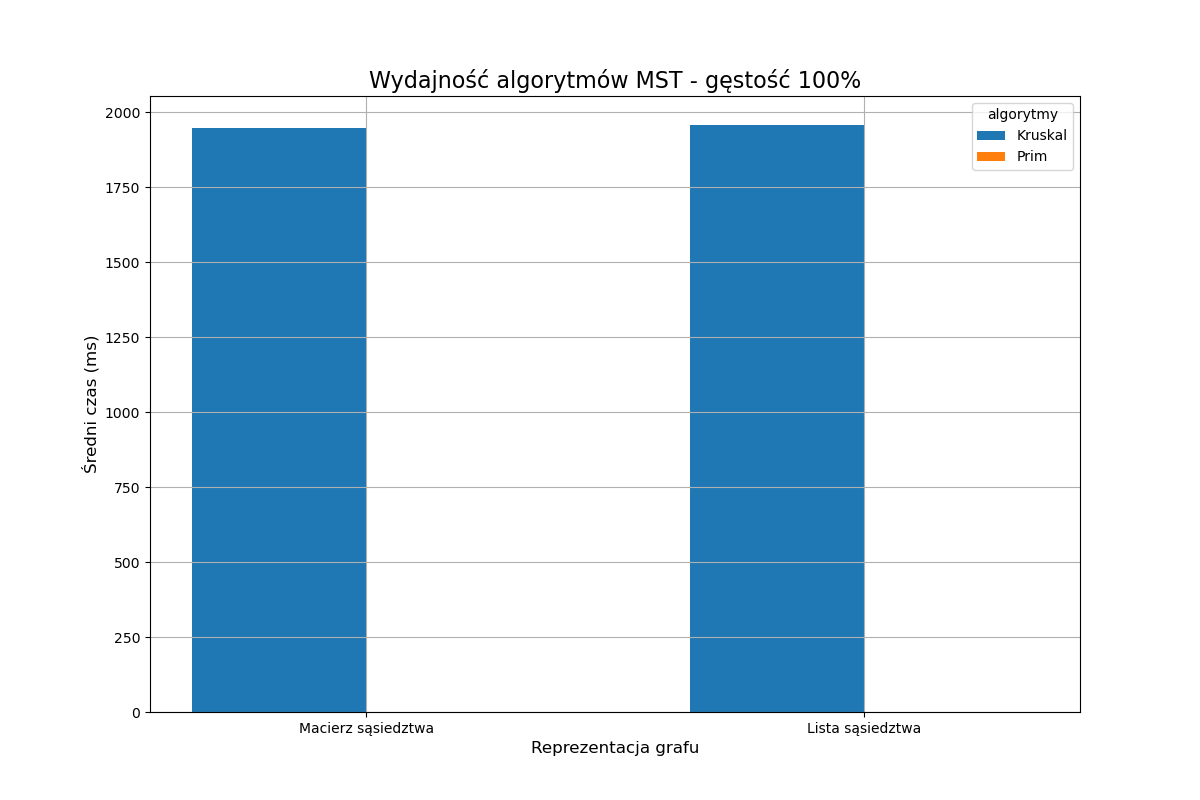
\includegraphics[scale=0.5]{../Python/charts_type2/Typ2_MST_gestosc100_wykres.png}
    \caption{Czasy wykonania algorytmów Kruskala i Prima dla gęstości 100\%}
\end{figure}

\subsection{Problem najkrótszej ścieżki}

\subsubsection{Tabele}
\pgfplotstableread[col sep=comma]{../Results/Type1_SHORTEST_PATH_type1_AdjacencyList.csv}\datatable

\begin{table}[H]
\centering
\pgfplotstabletypeset[
    columns/column1/.style={column name=Density},
    columns/column2/.style={column name=Kruskal (ms)},
    columns/column3/.style={column name=Prim (ms)},
    every head row/.style={before row=\toprule,after row=\midrule},
    every last row/.style={after row=\bottomrule}
]{\datatable}
\caption{Tabela średnich wyników w milisekundach dla algorytmu Dijkstry i Bellmana-Forda dla Listy sąsiedztwa}
\end{table}

\pgfplotstableread[col sep=comma]{../Results/Type1_SHORTEST_PATH_type1_AdjacencyMatrix.csv}\datatable

\begin{table}[H]
\centering
\pgfplotstabletypeset[
    columns/column1/.style={column name=Density},
    columns/column2/.style={column name=Kruskal (ms)},
    columns/column3/.style={column name=Prim (ms)},
    every head row/.style={before row=\toprule,after row=\midrule},
    every last row/.style={after row=\bottomrule}
]{\datatable}
\caption{Tabela średnich wyników w milisekundach dla algorytmu Dijkstry i Bellmana-Forda dla Macierzy sąsiedztwa}
\end{table}

\subsubsection{Wykresy Typu 1 dla Dijkstry i Bellmana-Forda}

\begin{figure}[H]
    \centering
    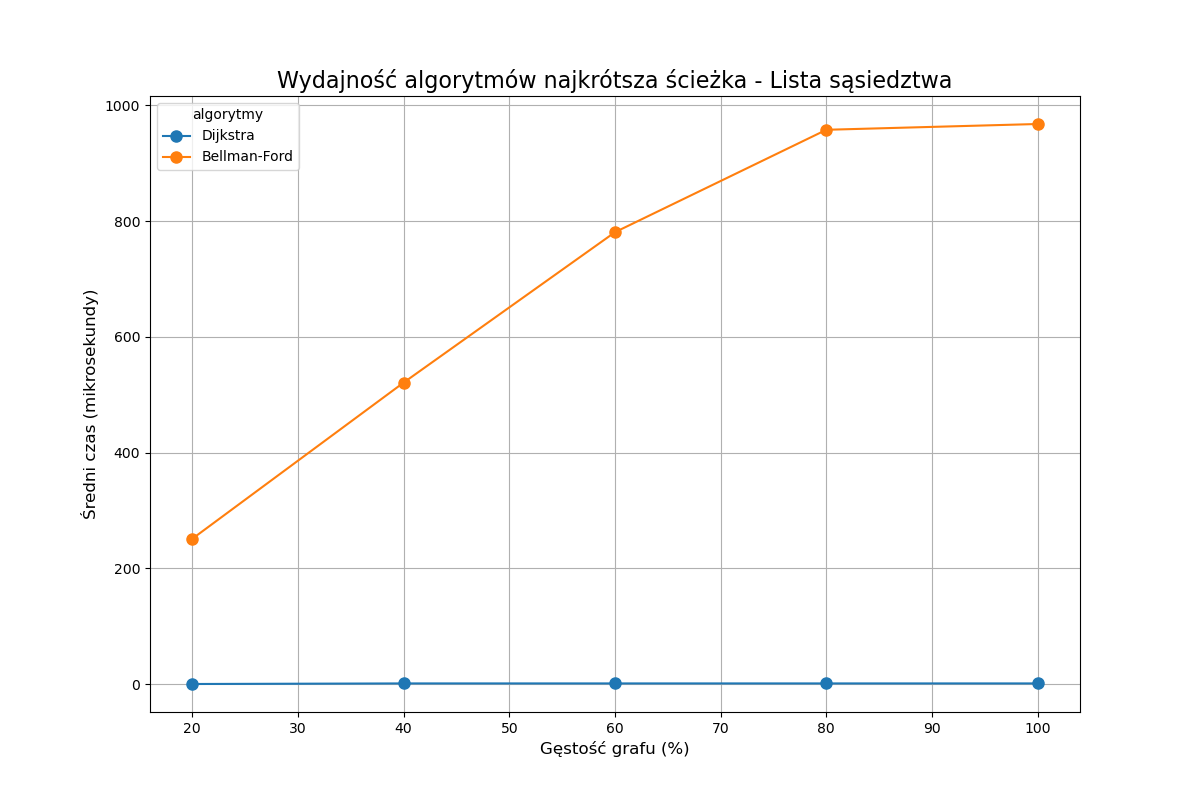
\includegraphics[scale=0.5]{../Python/charts_type1/Typ1_SHORTEST_PATH_Lista_sąsiedztwa_wykres.png}
    \caption{Czasy wykonania algorytmów Dijkstry i Bellmana-Forda dla Listy sąsiedztwa}
\end{figure}
\begin{figure}[H]
    \centering
    \includegraphics[scale=0.5]{../Python/charts_type1/Typ1_SHORTEST_PATH_Macierz_sąsiedztwa_wykres.png}
    \caption{Czasy wykonania algorytmów Dijkstry i Bellmana-Forda dla Macierzy sąsiedztwa}
\end{figure}

\subsubsection{Wykresy Typu 2 dla Dijkstry i Bellmana-Forda}

\begin{figure}[H]
    \centering
    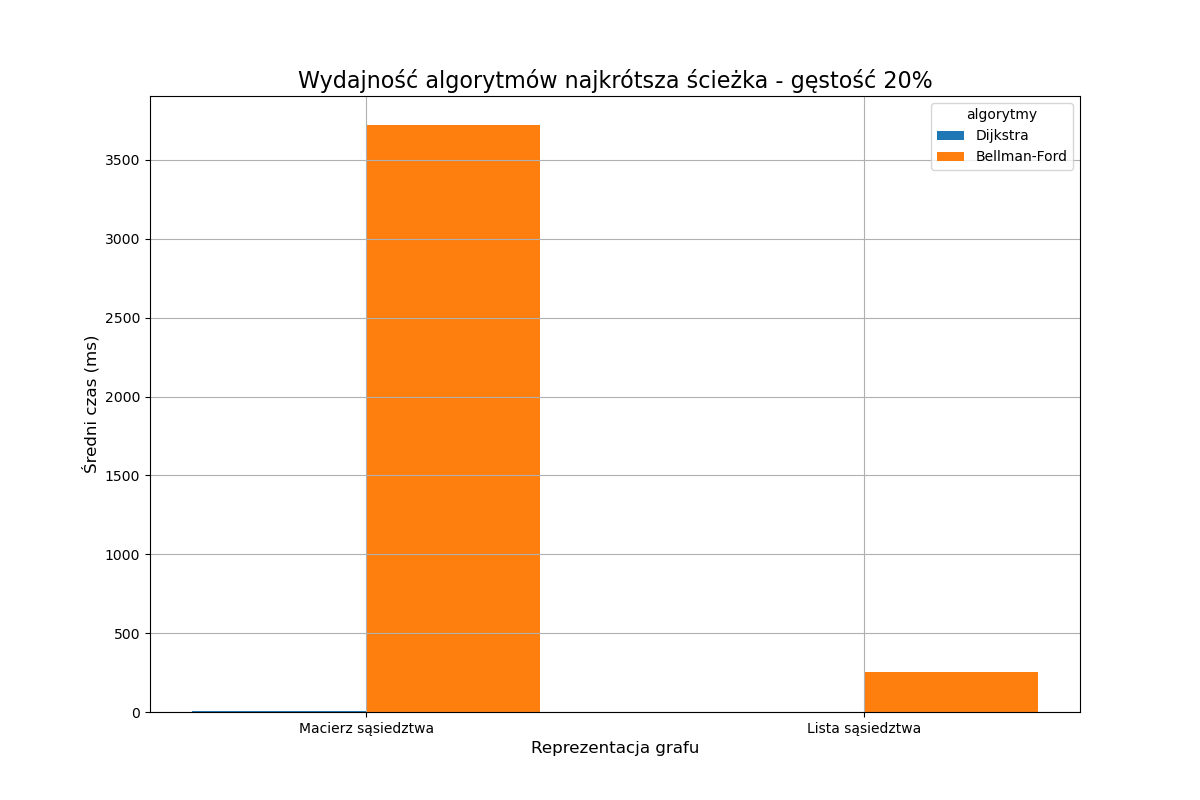
\includegraphics[scale=0.5]{../Python/charts_type2/Typ2_SHORTEST_PATH_gestosc20_wykres.png}
    \caption{Czasy wykonania algorytmów Dijkstry i Bellmana-Forda dla gęstości 20\%}
\end{figure}
\begin{figure}[H]
    \centering
    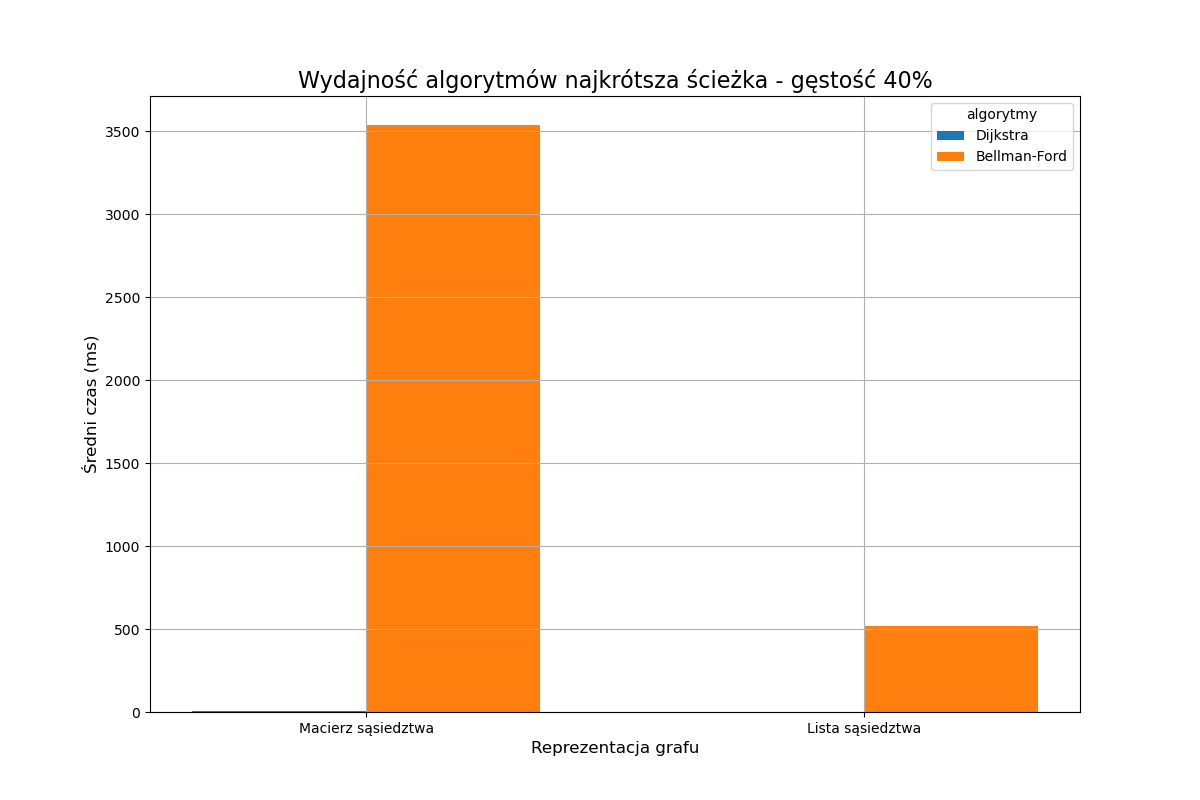
\includegraphics[scale=0.5]{../Python/charts_type2/Typ2_SHORTEST_PATH_gestosc40_wykres.png}
    \caption{Czasy wykonania algorytmów Dijkstry i Bellmana-Forda dla gęstości 40\%}
\end{figure}

\begin{figure}[H]
    \centering
    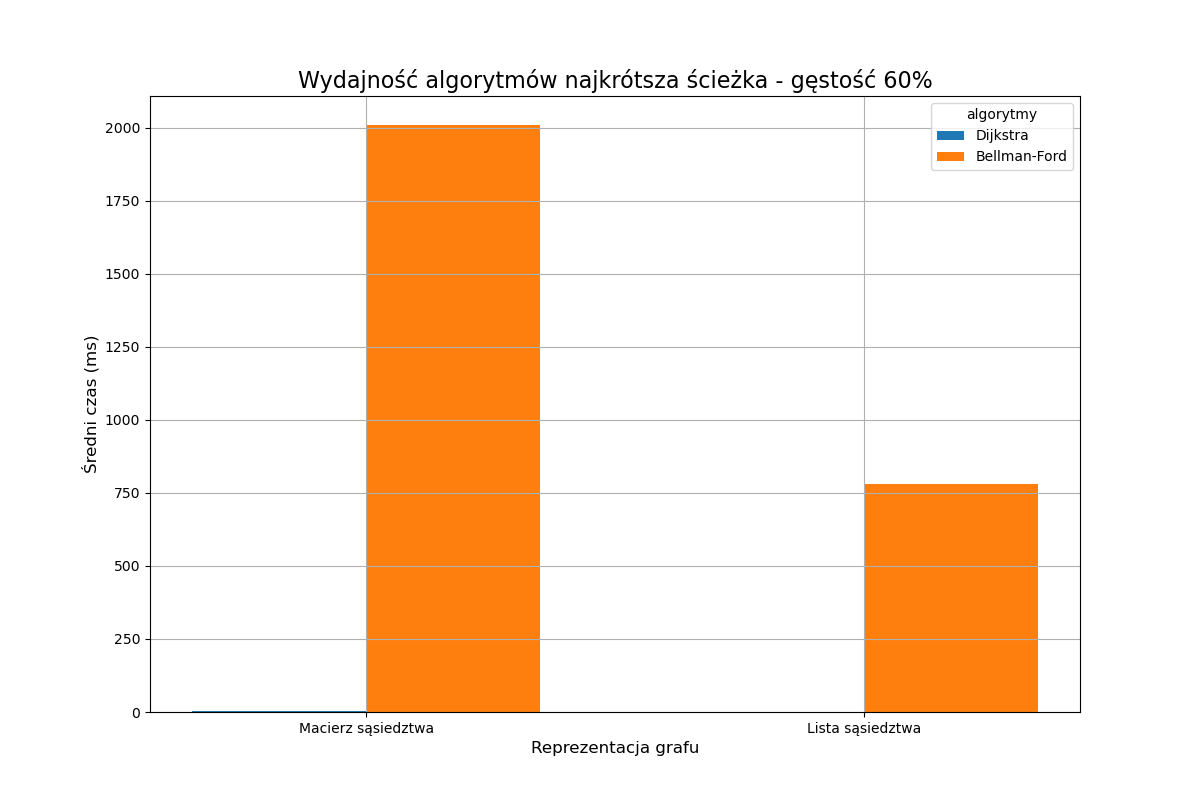
\includegraphics[scale=0.5]{../Python/charts_type2/Typ2_SHORTEST_PATH_gestosc60_wykres.png}
    \caption{Czasy wykonania algorytmów Dijkstry i Bellmana-Forda dla gęstości 60\%}
\end{figure}

\begin{figure}[H]
    \centering
    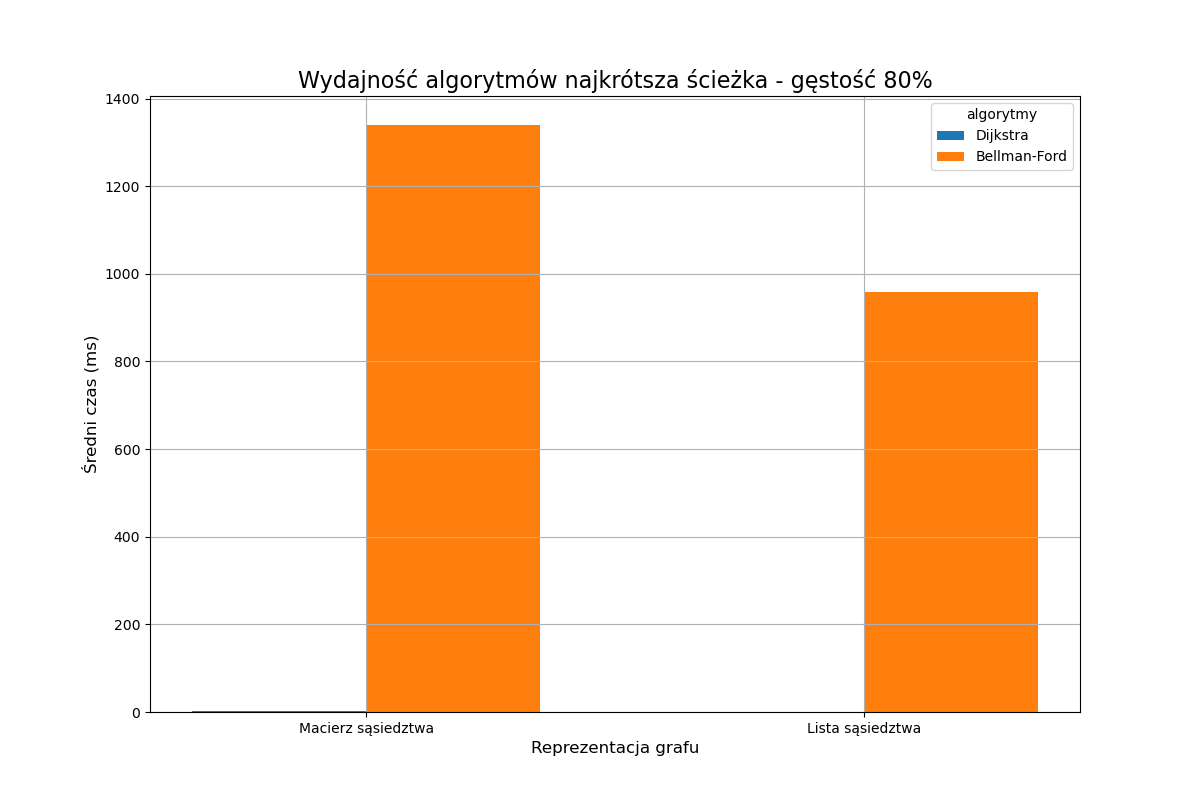
\includegraphics[scale=0.5]{../Python/charts_type2/Typ2_SHORTEST_PATH_gestosc80_wykres.png}
    \caption{Czasy wykonania algorytmów Dijkstry i Bellmana-Forda dla gęstości 80\%}
\end{figure}

\begin{figure}[H]
    \centering
    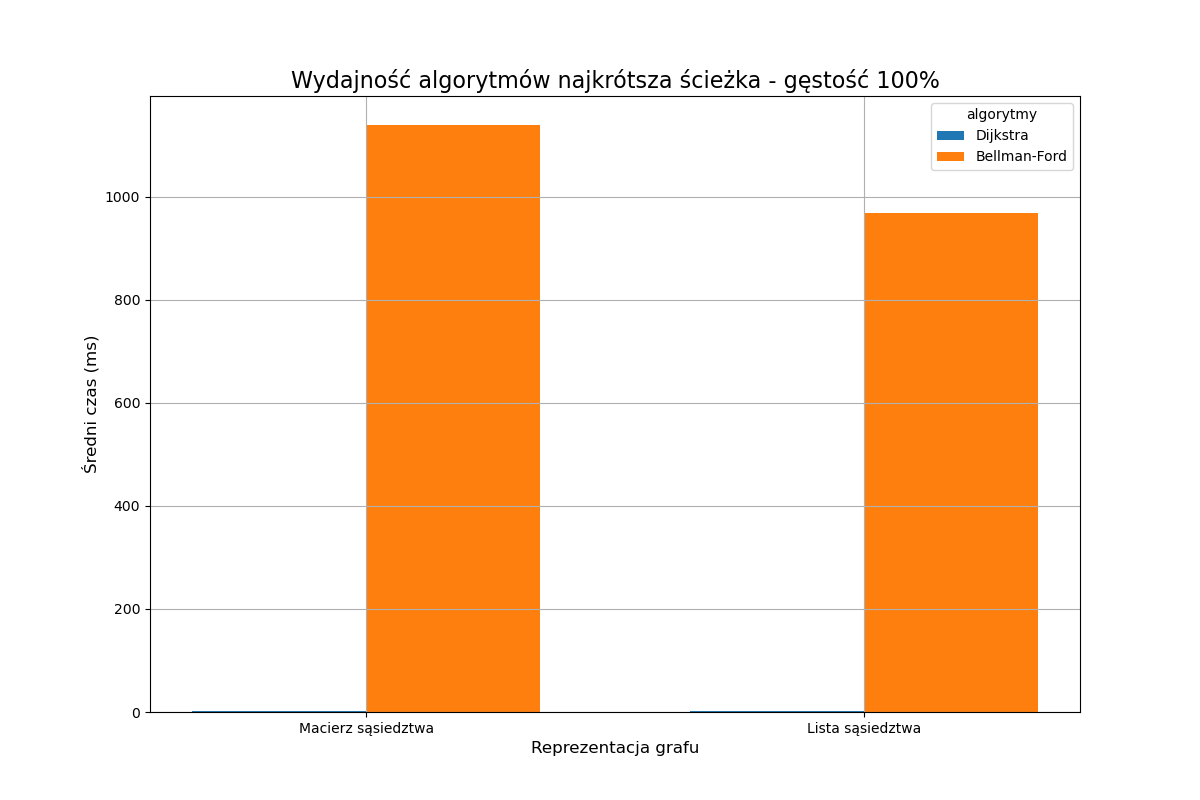
\includegraphics[scale=0.5]{../Python/charts_type2/Typ2_SHORTEST_PATH_gestosc100_wykres.png}
    \caption{Czasy wykonania algorytmów Dijkstry i Bellmana-Forda dla gęstości 100\%}
\end{figure}

\subsection{Problem maksymalnego przepływu}

\subsubsection{Tabele}
\pgfplotstableread[col sep=comma]{../Results/Type1_MAX_FLOW_type1_AdjacencyList.csv}\datatable

\begin{table}[H]
\centering
\pgfplotstabletypeset[
    columns/column1/.style={column name=Density},
    columns/column2/.style={column name=Kruskal (ms)},
    columns/column3/.style={column name=Prim (ms)},
    every head row/.style={before row=\toprule,after row=\midrule},
    every last row/.style={after row=\bottomrule}
]{\datatable}
\caption{Tabela średnich wyników w milisekundach dla algorytmu Forda-Fulkersona i Edmondsa-Karpa dla Listy sąsiedztwa}
\end{table}

\pgfplotstableread[col sep=comma]{../Results/Type1_MAX_FLOW_type1_AdjacencyMatrix.csv}\datatable

\begin{table}[H]
\centering
\pgfplotstabletypeset[
    columns/column1/.style={column name=Density},
    columns/column2/.style={column name=Kruskal (ms)},
    columns/column3/.style={column name=Prim (ms)},
    every head row/.style={before row=\toprule,after row=\midrule},
    every last row/.style={after row=\bottomrule}
]{\datatable}
\caption{Tabela średnich wyników w milisekundach dla algorytmu Forda-Fulkersona i Edmondsa-Karpa dla Macierzy sąsiedztwa}
\end{table}

\subsubsection{Wykresy Typu 1 dla Forda-Fulkersona i Edmondsa-Karpa}

\begin{figure}[H]
    \centering
    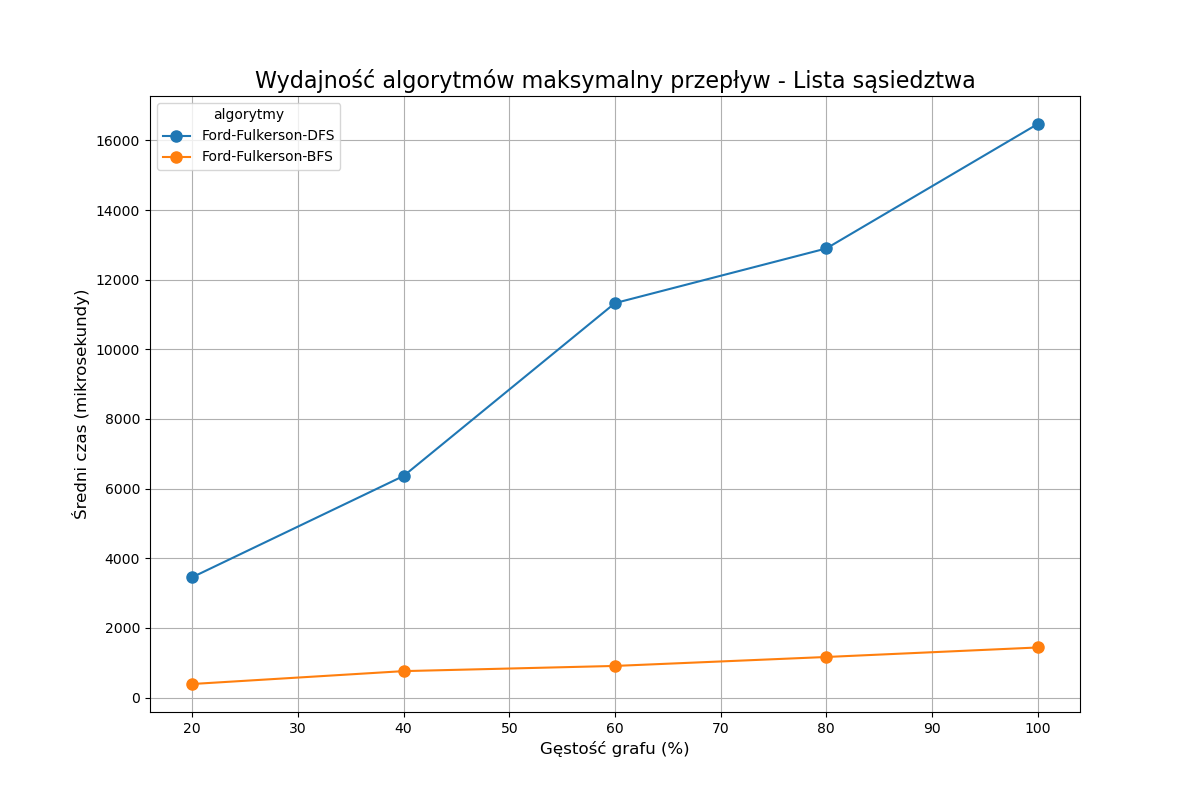
\includegraphics[scale=0.5]{../Python/charts_type1/Typ1_MAX_FLOW_Lista_sąsiedztwa_wykres.png}
    \caption{Czasy wykonania algorytmów Forda-Fulkersona i Edmondsa-Karpa dla Listy sąsiedztwa}
\end{figure}
\begin{figure}[H]
    \centering
    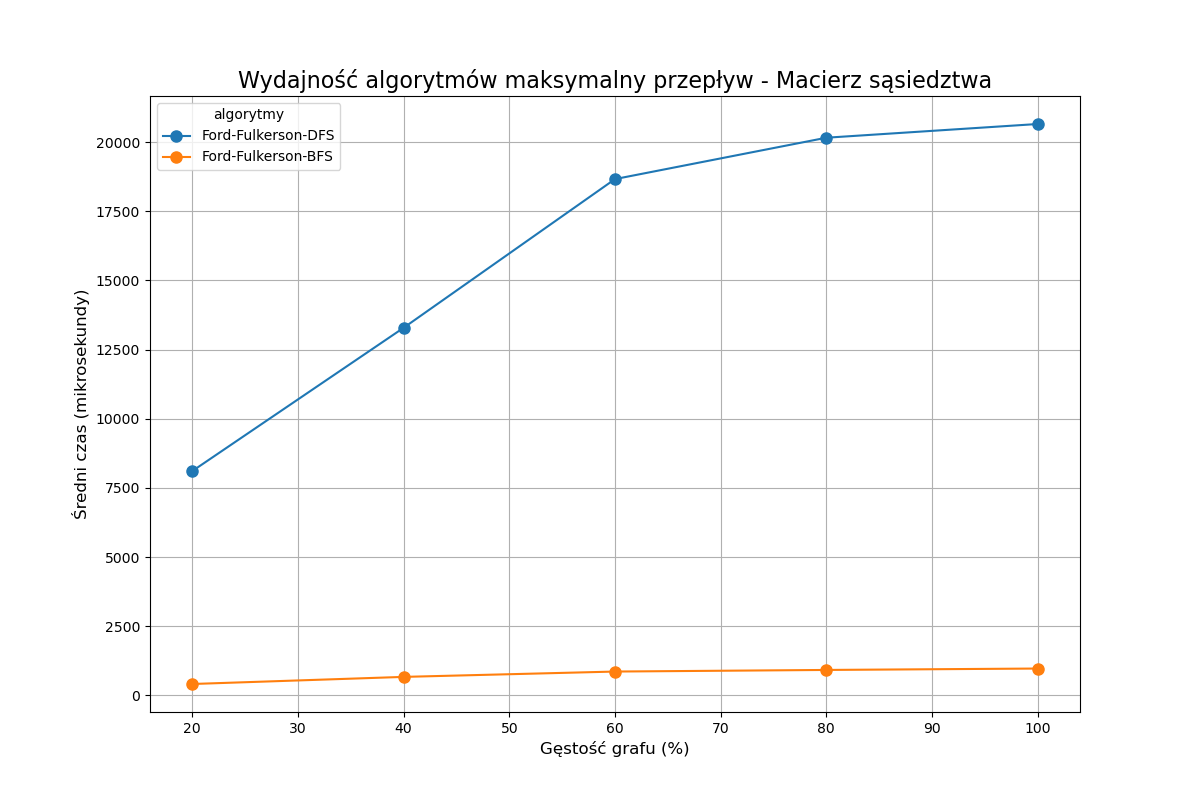
\includegraphics[scale=0.5]{../Python/charts_type1/Typ1_MAX_FLOW_Macierz_sąsiedztwa_wykres.png}
    \caption{Czasy wykonania algorytmów Forda-Fulkersona i Edmondsa-Karpa dla Macierzy sąsiedztwa}
\end{figure}

\subsubsection{Wykresy Typu 2 dla Forda-Fulkersona i Edmondsa-Karpa}

\begin{figure}[H]
    \centering
    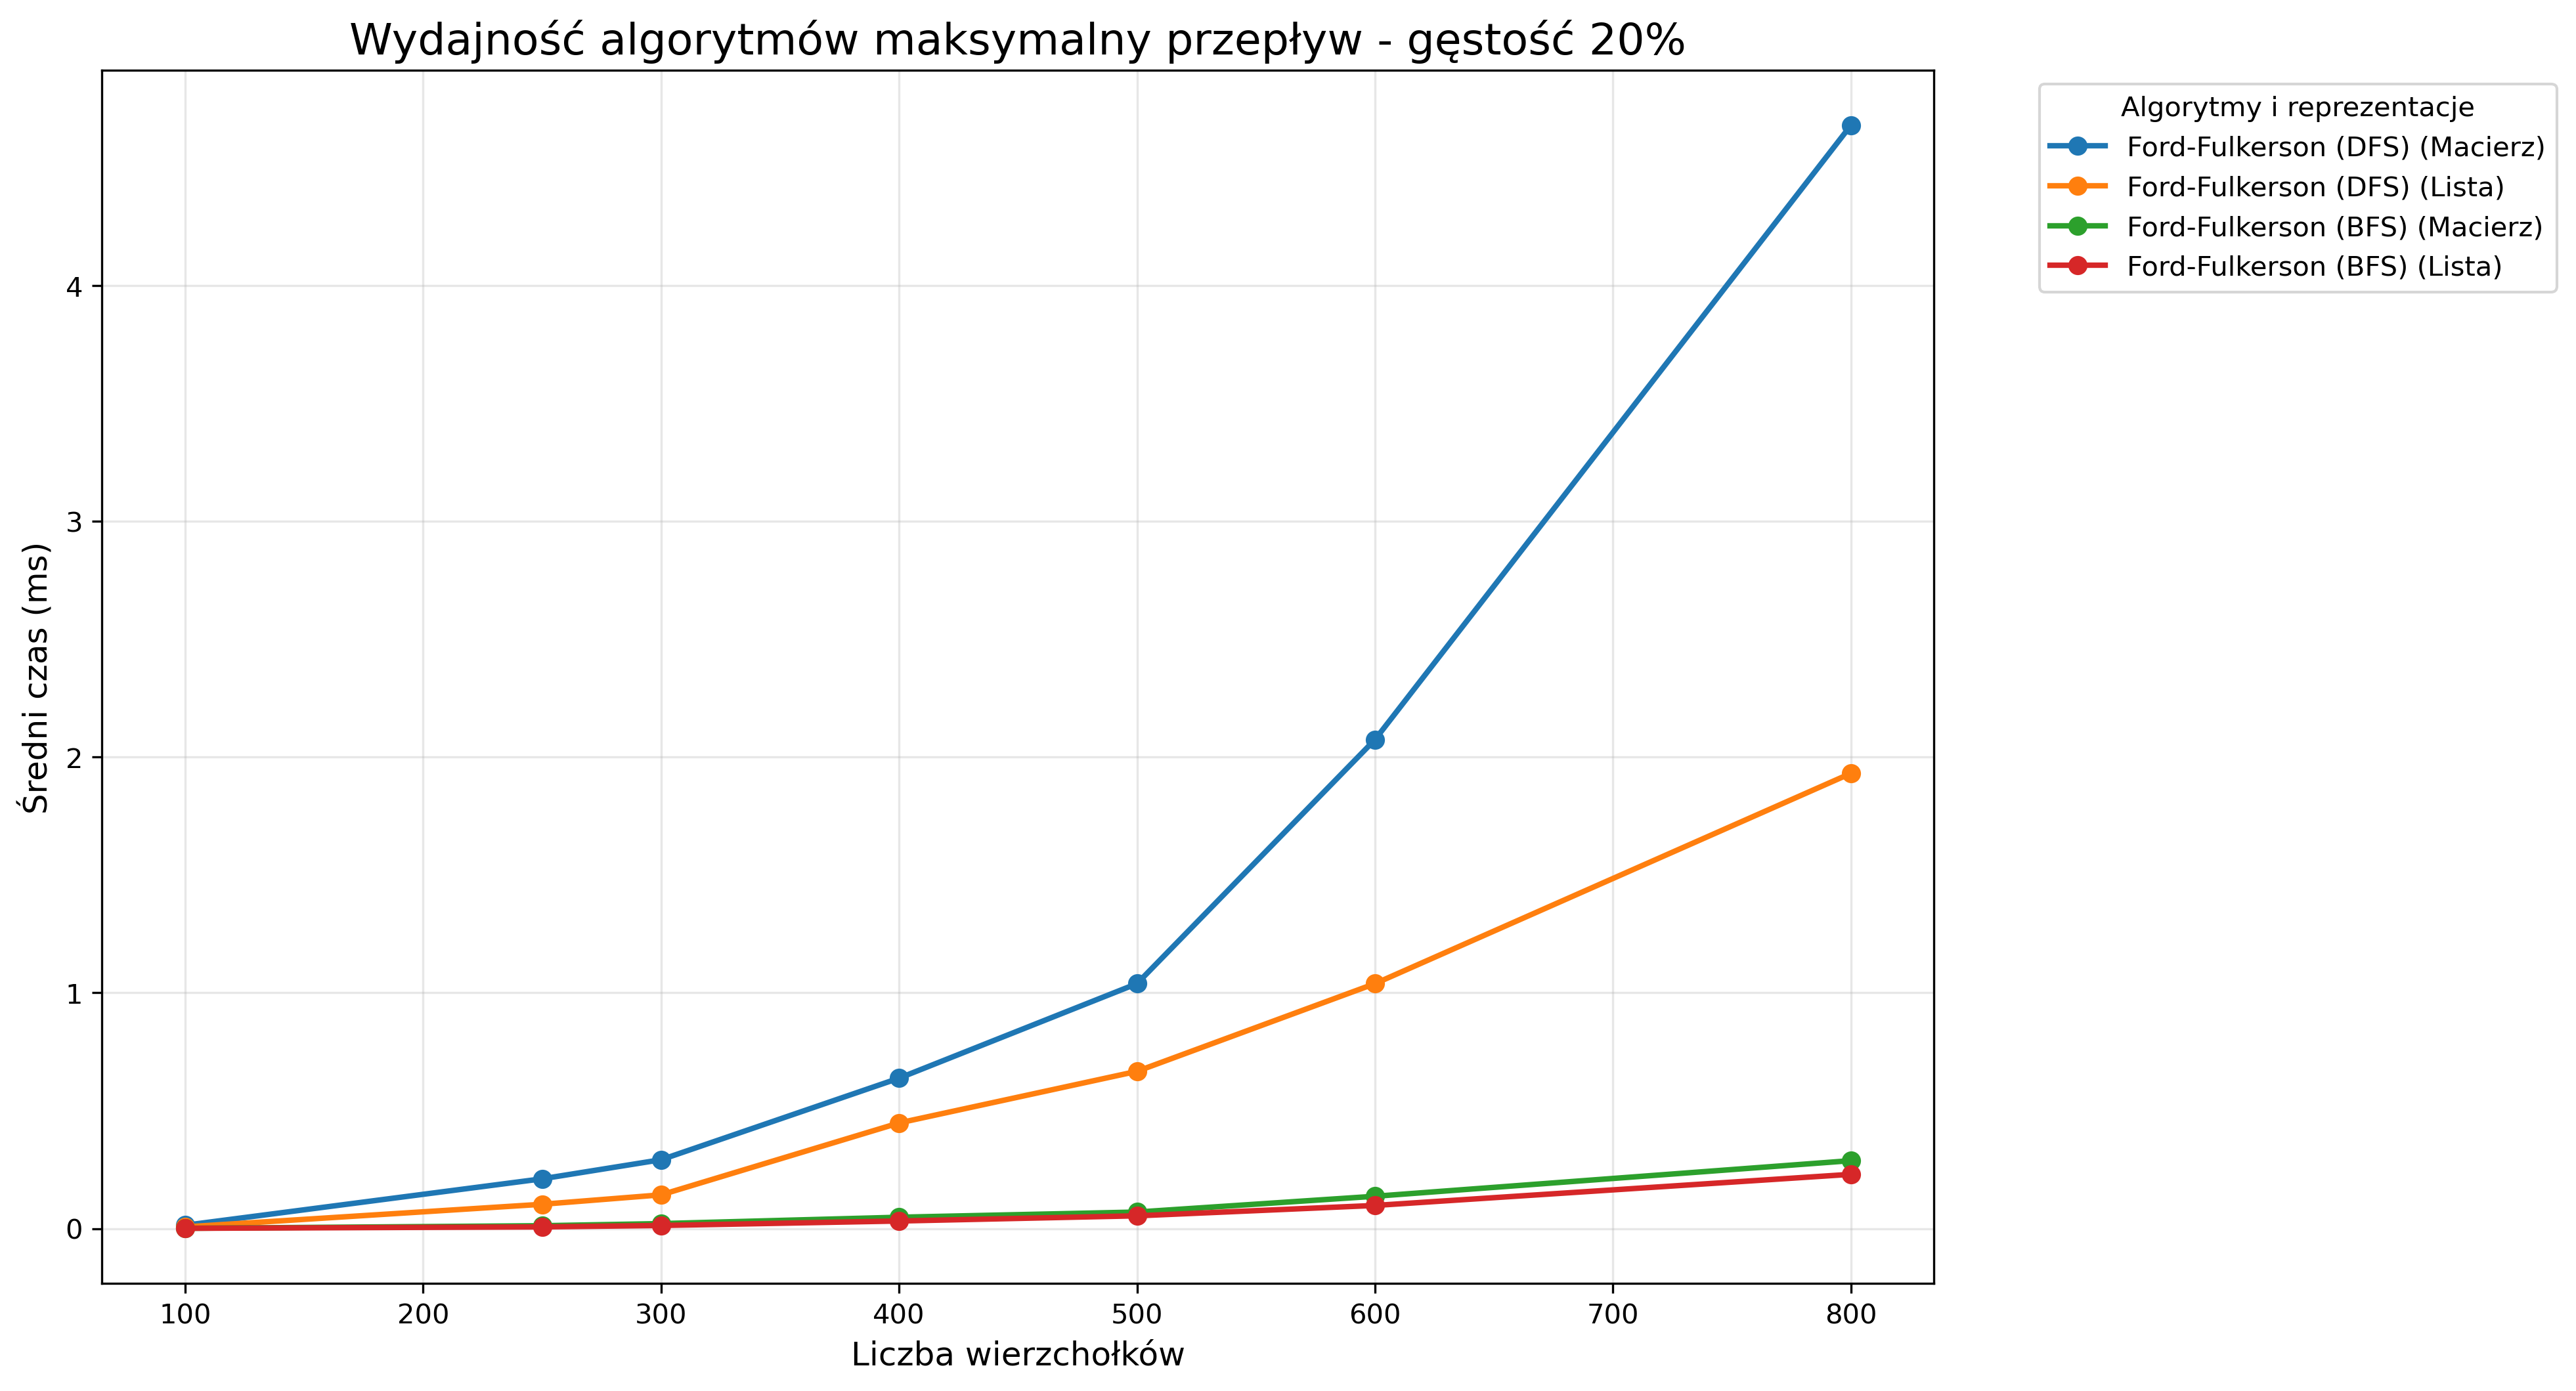
\includegraphics[scale=0.5]{../Python/charts_type2/Typ2_MAX_FLOW_gestosc20_wykres.png}
    \caption{Czasy wykonania algorytmów Forda-Fulkersona i Edmondsa-Karpa dla gęstości 20\%}
\end{figure}
\begin{figure}[H]
    \centering
    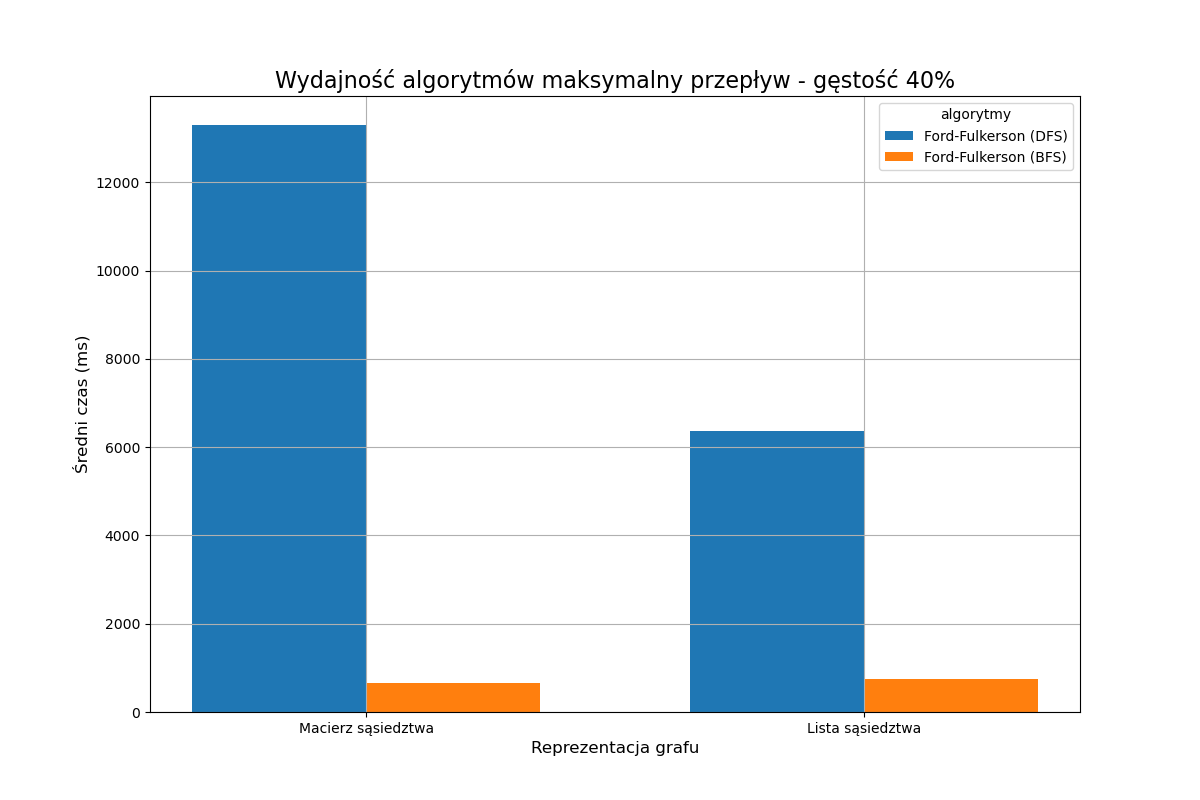
\includegraphics[scale=0.5]{../Python/charts_type2/Typ2_MAX_FLOW_gestosc40_wykres.png}
    \caption{Czasy wykonania algorytmów Forda-Fulkersona i Edmondsa-Karpa dla gęstości 40\%}
\end{figure}

\begin{figure}[H]
    \centering
    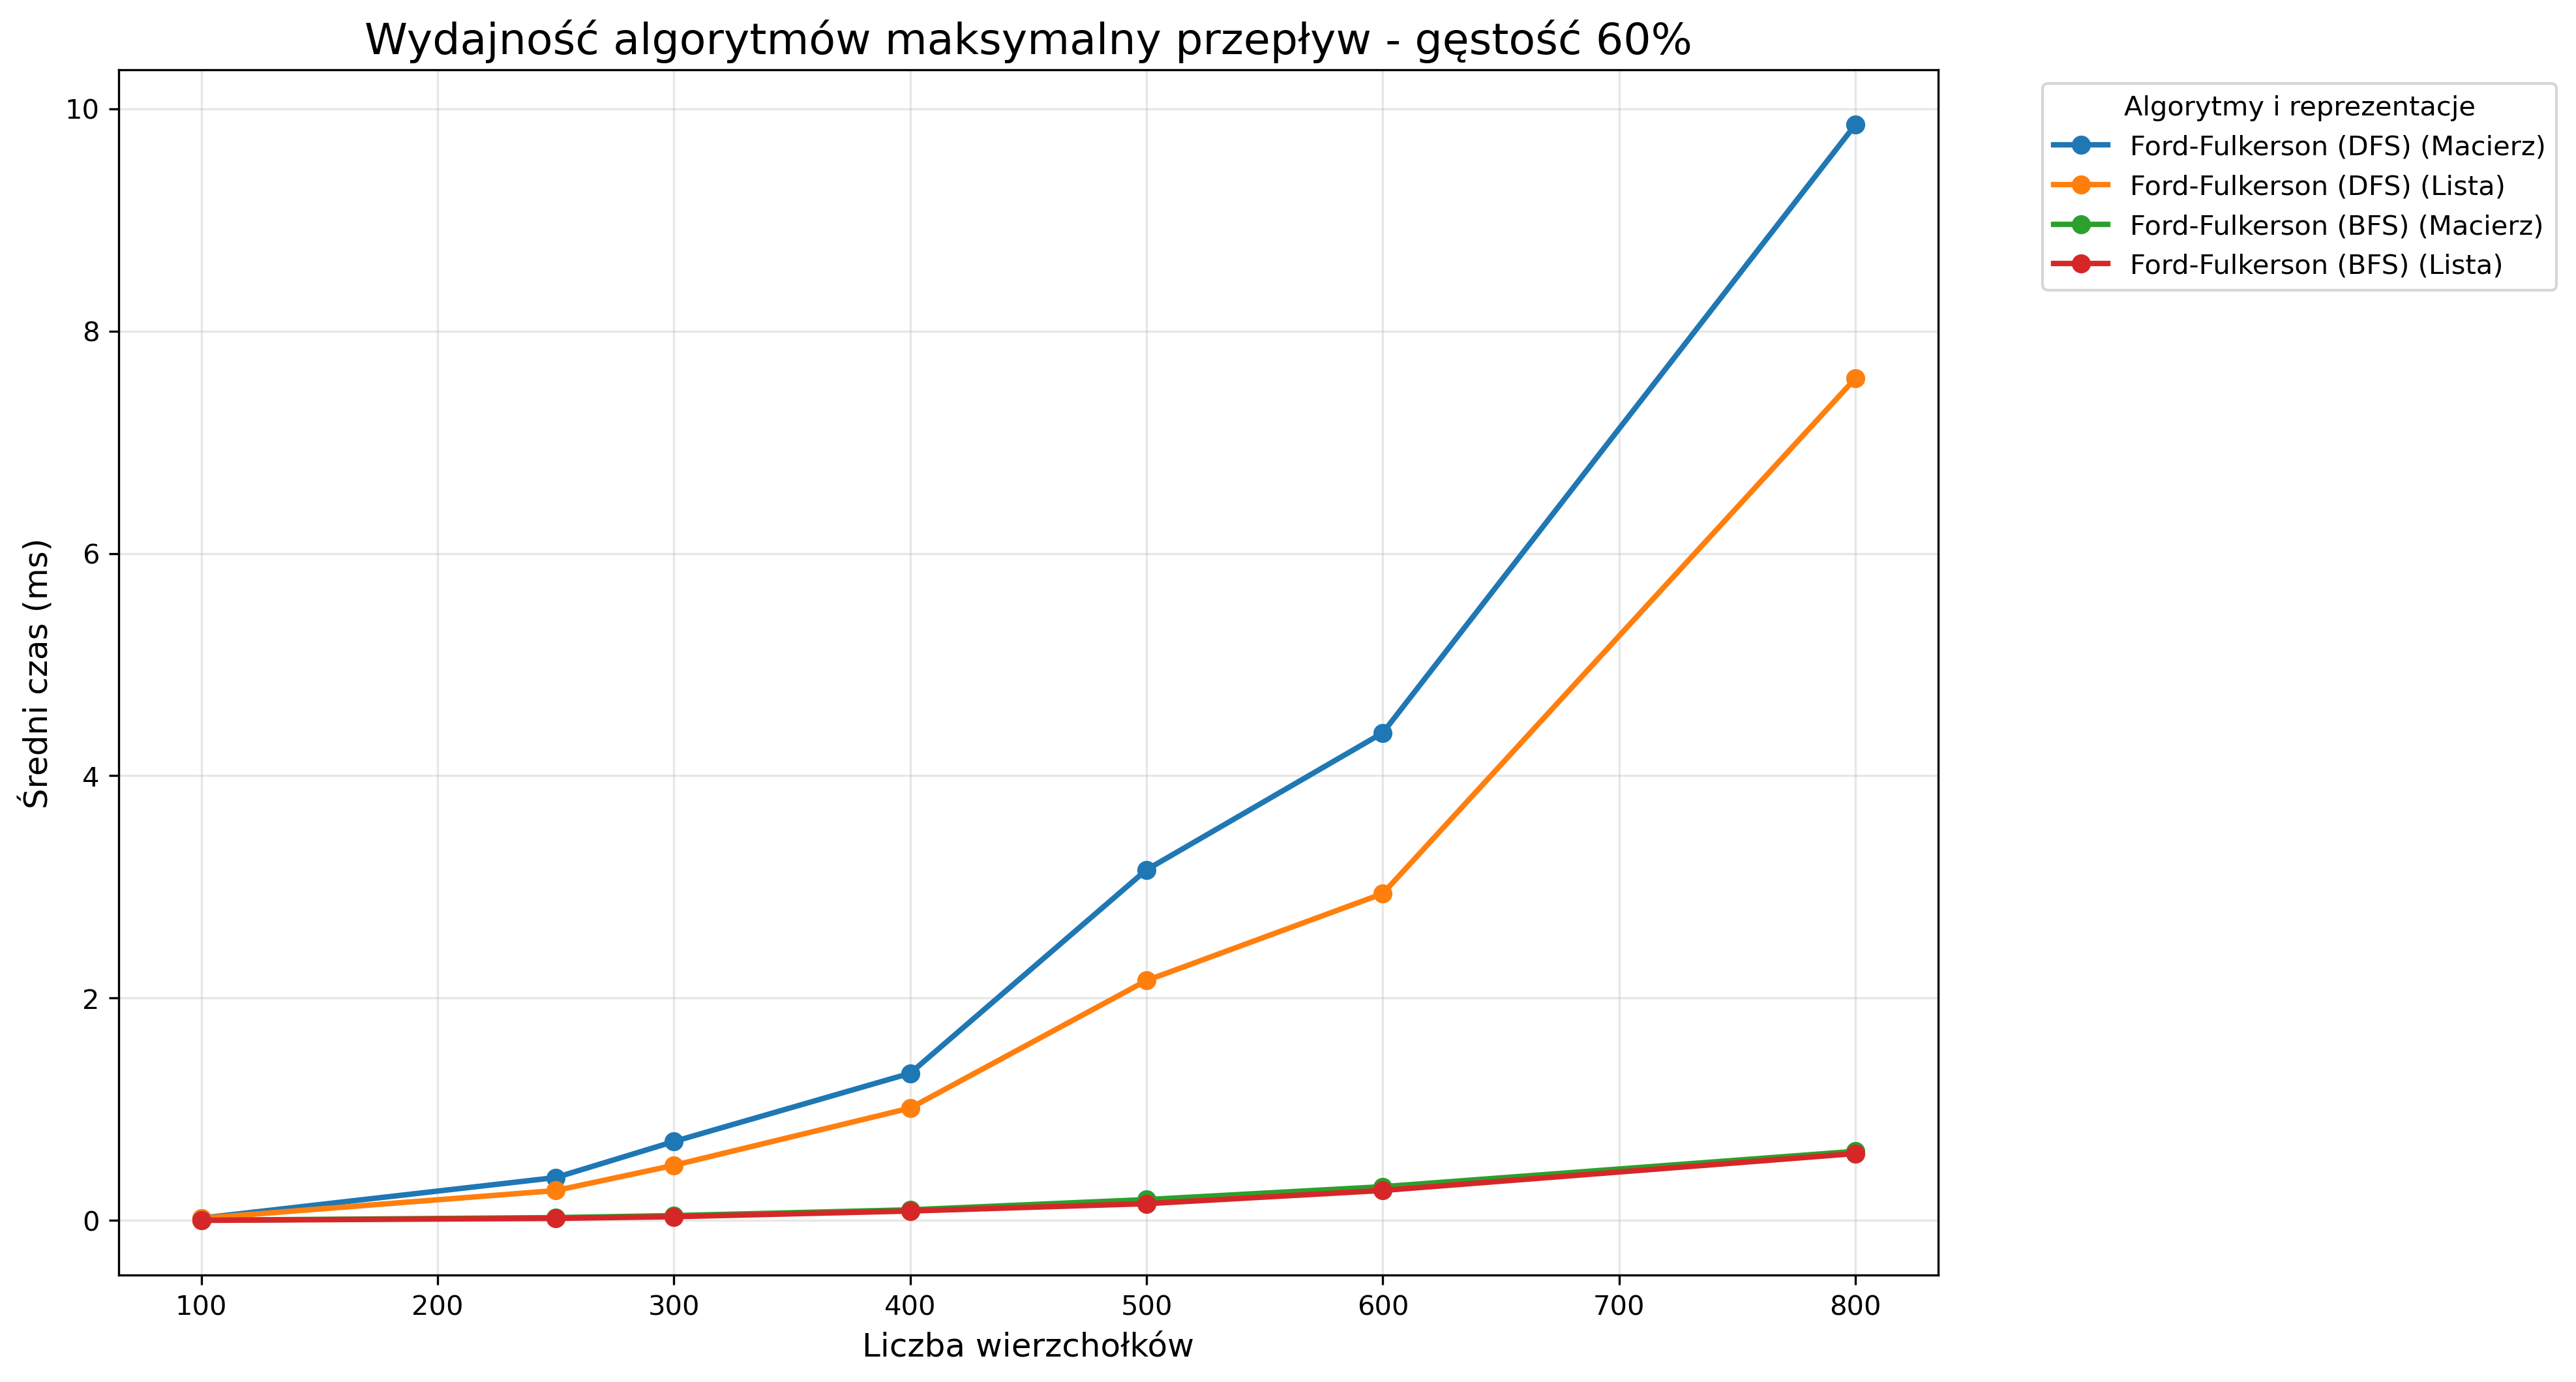
\includegraphics[scale=0.5]{../Python/charts_type2/Typ2_MAX_FLOW_gestosc60_wykres.png}
    \caption{Czasy wykonania algorytmów Forda-Fulkersona i Edmondsa-Karpa dla gęstości 60\%}
\end{figure}

\begin{figure}[H]
    \centering
    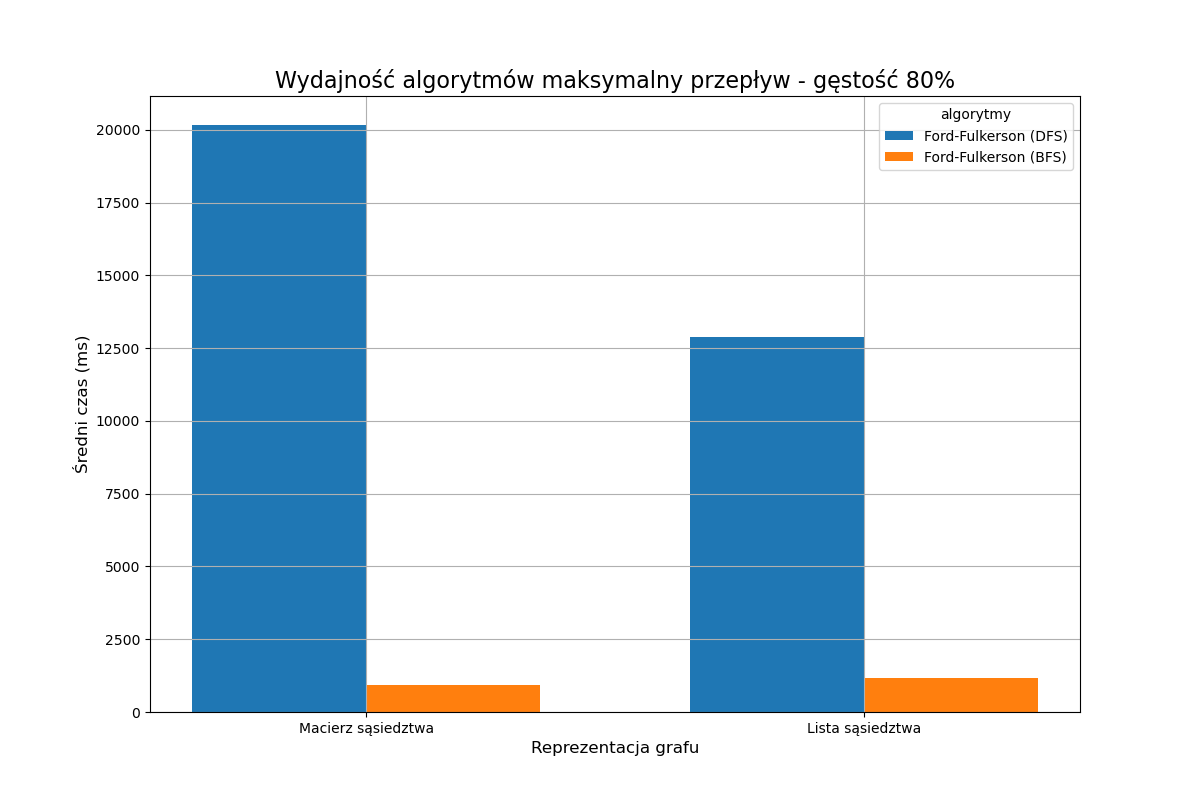
\includegraphics[scale=0.5]{../Python/charts_type2/Typ2_MAX_FLOW_gestosc80_wykres.png}
    \caption{Czasy wykonania algorytmów Forda-Fulkersona i Edmondsa-Karpa dla gęstości 80\%}
\end{figure}

\begin{figure}[H]
    \centering
    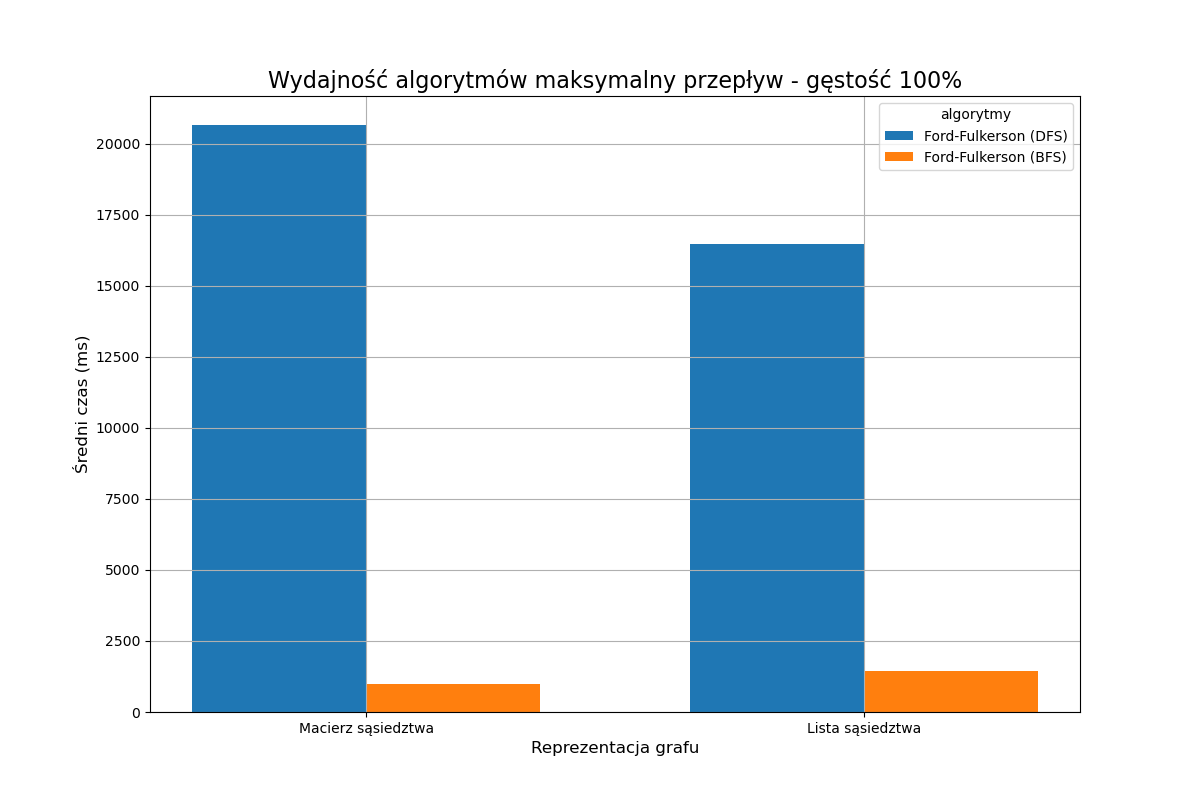
\includegraphics[scale=0.5]{../Python/charts_type2/Typ2_MAX_FLOW_gestosc100_wykres.png}
    \caption{Czasy wykonania algorytmów Forda-Fulkersona i Edmondsa-Karpa dla gęstości 100\%}
\end{figure}

\section{Podsumowanie}

Na podstawie eksperymentu można zauważyć, iż czasy wykonania algorytmów dla różnych reprezentacji oraz gęstości potrafią drastycznie się różnić.
W przypadku problemu MST algorytm Prima jest zdecydowanie szybszy niż algorytm Kruskala, co jest spowodowane tym, że algorytm Prima działa w czasie $O(E \log V)$, podczas gdy algorytm Kruskala w czasie $O(E \log E)$.
Jednakże ta różnica nie powinna być rzędu setek i może to wynikać z różnych zaburzeń wynikających z metody pomiaru czasu wykonania algorytmu, takich jak obciążenie procesora, czy też inne procesy działające w tle.
Podobne różnice widać w przypadku problemów najkrótszej ścieżki oraz maksymalnego przepływu, gdzie algorytm Dijkstry jest szybszy niż algorytm Bellmana-Forda, a algorytm Edmondsa-Karpa jest szybszy niż algorytm Forda-Fulkersona.
Te różnice również sięgają podobnej skali co w wypadku problemu MST. 

Kolejne ciekawe zjawiska można także zauważyć w wykonaniu algorytmu Kruskala i Prima na różnych reprezentacjach grafu.
W przypadku listy sąsiedztwa czas wykonania algorytmu kruskala, czas ten rośnie dla coraz większych gęstości grafu, by potem spaść dla 100\% gęstości.
Takie zjawisko nie występuje w przypadku macierzy sąsiedztwa, gdzie czas wykonania algorytmu Kruskala rośnie wraz z gęstością grafu. Podobne zjawisko występuje dla algorytmu
Bellmana-Forda, gdzie gdy gęstość grafu rośnie, czas wykonania spada.

Wyniki jasno pokazują, które algorytmy sprawdzą się najlepiej w każdym wymienionym problemie i poza przypadkami tzw. granicznymi, w większości będą one używane.
\section{Literatura}
\begin{itemize}
    \item Opracowaie tabel: praca własna, dane obrobione przez skrypty w języku $Python$
    \item Dokumentacja chrono: \url{https://cplusplus.com/reference/chrono/}
    \item Dokumentacja fstream \url{https://cplusplus.com/reference/fstream/}
    \item Opracowanie algorytmów MST \url{https://eduinf.waw.pl/inf/alg/001_search/0141.php}
    \item Opracowanie algorytmów SSP \\ \url{https://eduinf.waw.pl/inf/alg/001_search/0138.php} \\ \url{https://eduinf.waw.pl/inf/alg/001_search/0138a.php}
    \item Opracowanie algorytmów Maksymalnego przepływu: \\ \url{https://eduinf.waw.pl/inf/alg/001_search/0125.php} \\ \url{https://eduinf.waw.pl/inf/alg/001_search/0126.php}
    \item Złożoność pamięciowa reprezentacji grafów: \textit{T. H. Cormen - Wprowadzenie do algorytmów, str. 591-593}
\end{itemize}

\end{document}